%==============================================================================
% Chapitre 63 - Les matériaux des projectiles de chasse
%==============================================================================

\section{Introduction}

Les performances d'un projectile dépendent non seulement de sa forme mais
également du matériau qui le compose.

La densité, la dureté et le coût influencent directement les caractéristiques
des munitions.

\begin{aretenir}

Le matériau d'un projectile influence sa masse, son comportement en vol et ses
performances terminales.

\end{aretenir}

\section{Le plomb}

Le plomb a longtemps constitué le matériau de référence pour les projectiles de
chasse.

Ses propriétés expliquent largement son succès historique.

\section{Avantages du plomb}

Le plomb présente plusieurs avantages :

\begin{itemize}
    \item densité élevée ;
    \item facilité de mise en forme ;
    \item coût relativement faible ;
    \item comportement bien connu.
\end{itemize}

\section{Densité et masse}

La densité élevée du plomb permet d'obtenir une masse importante dans un volume
réduit.

Cette caractéristique favorise la conservation de l'énergie au cours du vol.

\begin{figure}[htbp]
\centering

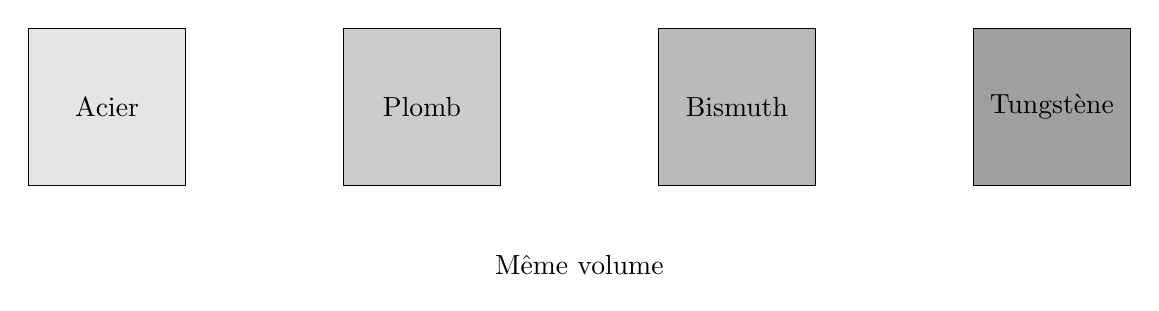
\begin{tikzpicture}

% Acier
\draw[fill=gray!20] (0,0) rectangle (2,2);
\node at (1,1) {Acier};

% Plomb
\draw[fill=gray!40] (4,0) rectangle (6,2);
\node at (5,1) {Plomb};

% Bismuth
\draw[fill=gray!55] (8,0) rectangle (10,2);
\node at (9,1) {Bismuth};

% Tungstène
\draw[fill=gray!75] (12,0) rectangle (14,2);
\node at (13,1) {Tungstène};

\node at (7,-1)
{Même volume};

\end{tikzpicture}

\caption{À volume égal, la masse dépend du matériau utilisé.}
\label{fig:volume_constant_materiaux}

\end{figure}

\section{Limites du plomb}

Malgré ses qualités, le plomb présente certaines limites.

Les préoccupations environnementales ont conduit à rechercher des matériaux de
substitution dans certaines applications.

\section{L'acier}

L'acier est aujourd'hui largement utilisé dans certaines cartouches à
grenaille.

Il constitue l'un des principaux matériaux alternatifs au plomb.

\section{Caractéristiques de l'acier}

Par rapport au plomb, l'acier présente généralement :

\begin{itemize}
    \item une densité plus faible ;
    \item une dureté plus importante ;
    \item un comportement différent dans le canon.
\end{itemize}

\section{Conséquences pratiques}

Pour une même taille de projectile, une bille d'acier possède généralement une
masse inférieure à celle d'une bille de plomb.

Cette différence influence les performances obtenues.

\section{Le bismuth}

Le bismuth est utilisé dans certaines munitions destinées à remplacer le
plomb.

Ses caractéristiques se rapprochent davantage de celles du plomb que celles de
l'acier.

\section{Le tungstène}

Le tungstène est l'un des matériaux les plus denses utilisés dans les
munitions modernes.

Il permet d'obtenir des projectiles particulièrement compacts pour une masse
donnée.

\begin{figure}[htbp]
\centering

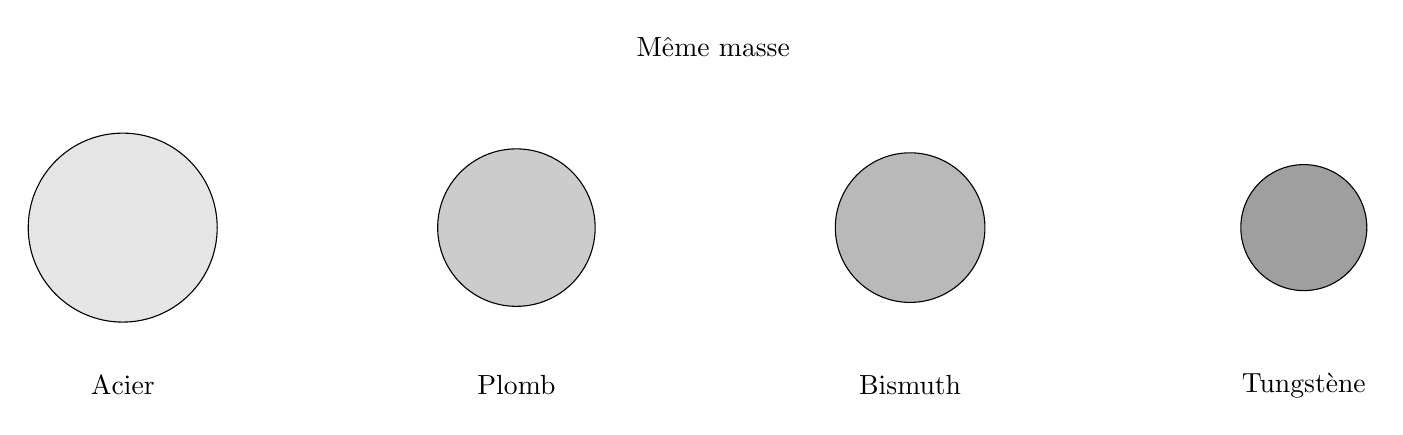
\begin{tikzpicture}

\draw[fill=gray!20] (0,0) circle (1.2);
\node at (0,-2)
{Acier};

\draw[fill=gray!40] (5,0) circle (1.0);
\node at (5,-2)
{Plomb};

\draw[fill=gray!55] (10,0) circle (0.95);
\node at (10,-2)
{Bismuth};

\draw[fill=gray!75] (15,0) circle (0.8);
\node at (15,-2)
{Tungstène};

\node at (7.5,2.3)
{Même masse};

\end{tikzpicture}

\caption{Pour une même masse, les matériaux plus denses occupent un volume plus faible.}
\label{fig:masse_constante_materiaux}

\end{figure}

\section{Avantages du tungstène}

Les projectiles contenant du tungstène présentent généralement :

\begin{itemize}
    \item une densité élevée ;
    \item une bonne conservation de l'énergie ;
    \item des performances élevées.
\end{itemize}

\section{Inconvénients du tungstène}

Le principal inconvénient du tungstène réside généralement dans son coût.

Cette caractéristique limite sa diffusion dans certaines applications.

\section{Influence sur la balistique}

À géométrie identique, le matériau influence :

\begin{itemize}
    \item la masse ;
    \item l'énergie ;
    \item le comportement en vol ;
    \item les effets à l'impact.
\end{itemize}

\begin{figure}[htbp]
\centering

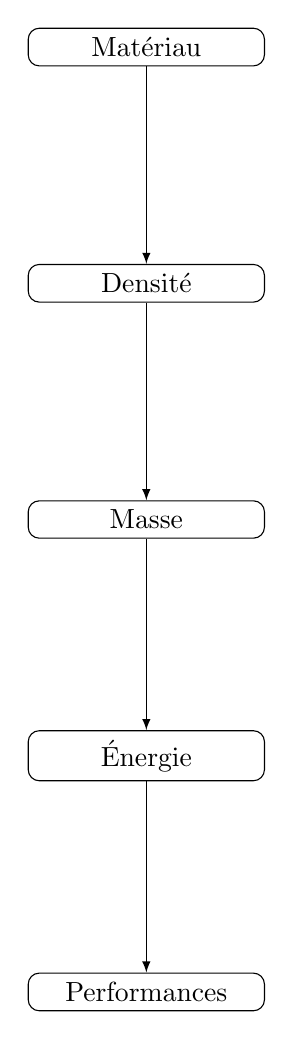
\begin{tikzpicture}[
every node/.style={
draw,
rounded corners,
align=center,
minimum width=3cm
}
]

\node (M) at (0,0)
{Matériau};

\node (D) at (0,-3)
{Densité};

\node (Ma) at (0,-6)
{Masse};

\node (E) at (0,-9)
{Énergie};

\node (P) at (0,-12)
{Performances};

\draw[-latex] (M) -- (D);
\draw[-latex] (D) -- (Ma);
\draw[-latex] (Ma) -- (E);
\draw[-latex] (E) -- (P);

\end{tikzpicture}

\caption{Influence simplifiée du matériau sur les performances du projectile.}
\label{fig:chaine_materiau_performances}

\end{figure}

\section{Compatibilité avec les armes}

Certains matériaux imposent des précautions particulières.

La compatibilité avec le canon et les chokes doit toujours être vérifiée.

\section{Évolution des réglementations}

Les réglementations applicables aux matériaux utilisés dans les munitions ont
évolué au fil du temps.

Ces évolutions ont contribué à l'apparition de nouvelles solutions.

\begin{figure}[htbp]
\centering

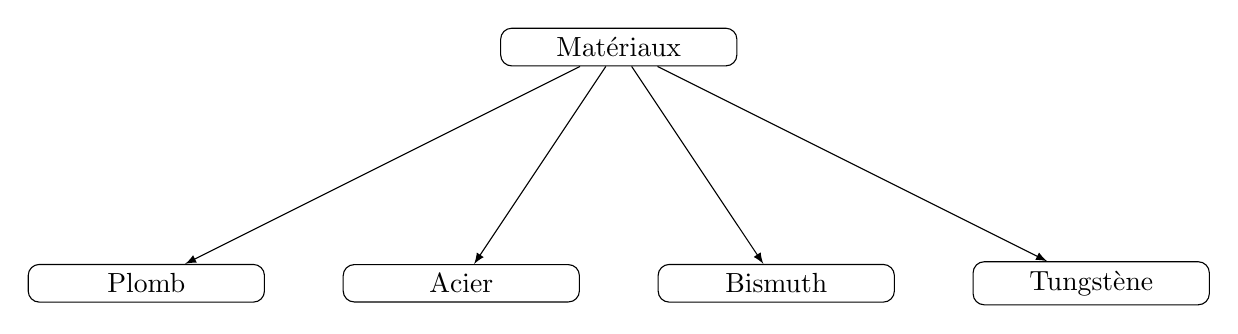
\begin{tikzpicture}[
every node/.style={
draw,
rounded corners,
align=center,
minimum width=3cm
}
]

\node (P) at (0,0)
{Matériaux};

\node (Pb) at (-6,-3)
{Plomb};

\node (Ac) at (-2,-3)
{Acier};

\node (Bi) at (2,-3)
{Bismuth};

\node (Tu) at (6,-3)
{Tungstène};

\draw[-latex] (P) -- (Pb);
\draw[-latex] (P) -- (Ac);
\draw[-latex] (P) -- (Bi);
\draw[-latex] (P) -- (Tu);

\end{tikzpicture}

\caption{Principaux matériaux utilisés pour les projectiles de chasse modernes.}
\label{fig:arbre_materiaux}

\end{figure}

\section{Choix du matériau}

Le choix dépend généralement :

\begin{itemize}
    \item de l'application ;
    \item des contraintes réglementaires ;
    \item du coût ;
    \item des performances recherchées.
\end{itemize}

\begin{figure}[htbp]
\centering

\begin{tikzpicture}

% Axes
\draw[-latex] (0,0) -- (10,0)
node[right] {Coût};

\draw[-latex] (0,0) -- (0,8)
node[above] {Performances};

% Points
\fill (2,2) circle (0.08);
\node[right] at (2,2) {Acier};

\fill (4,4) circle (0.08);
\node[right] at (4,4) {Plomb};

\fill (6,5) circle (0.08);
\node[right] at (6,5) {Bismuth};

\fill (8,7) circle (0.08);
\node[right] at (8,7) {Tungstène};

\end{tikzpicture}

\caption{Illustration qualitative des compromis entre coût et performances.}
\label{fig:compromis_materiaux}

\end{figure}

\begin{figure}[htbp]
\centering

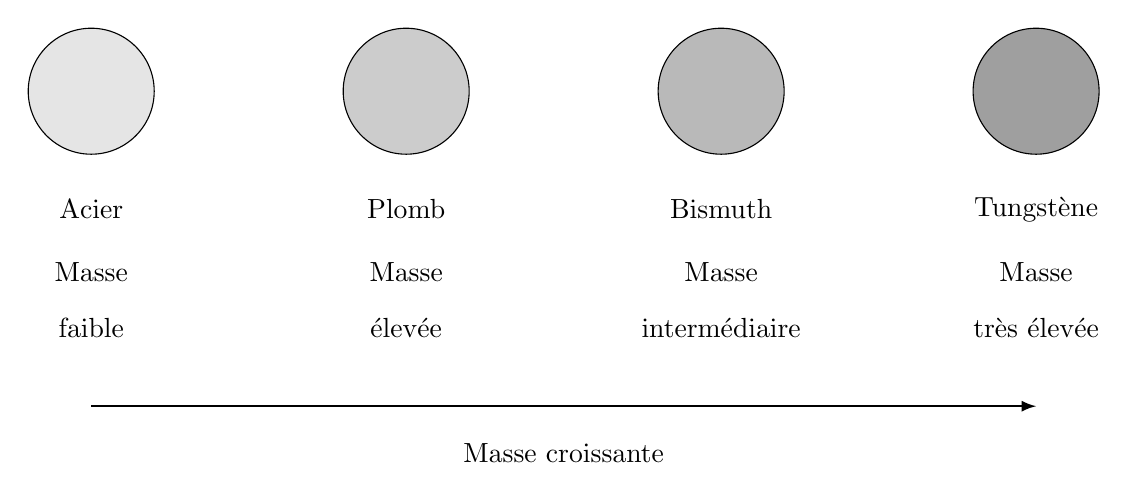
\begin{tikzpicture}

% Acier
\draw[fill=gray!20] (0,0) circle (0.8);

\node at (0,-1.5)
{Acier};

\node at (0,-2.3)
{Masse};

\node at (0,-3.0)
{faible};

% Plomb
\draw[fill=gray!40] (4,0) circle (0.8);

\node at (4,-1.5)
{Plomb};

\node at (4,-2.3)
{Masse};

\node at (4,-3.0)
{élevée};

% Bismuth
\draw[fill=gray!55] (8,0) circle (0.8);

\node at (8,-1.5)
{Bismuth};

\node at (8,-2.3)
{Masse};

\node at (8,-3.0)
{intermédiaire};

% Tungstène
\draw[fill=gray!75] (12,0) circle (0.8);

\node at (12,-1.5)
{Tungstène};

\node at (12,-2.3)
{Masse};

\node at (12,-3.0)
{très élevée};

\draw[-latex,thick]
(0,-4)
--
(12,-4);

\node at (6,-4.6)
{Masse croissante};

\end{tikzpicture}

\caption{À diamètre identique, la masse dépend directement du matériau utilisé.}
\label{fig:diametre_identique_masse_variable}

\end{figure}

\section{Vers les désignations commerciales}

Les matériaux ne constituent qu'une partie des informations figurant sur une
boîte de cartouches.

Le chapitre suivant examinera la lecture des désignations commerciales.

\section{À retenir}

\begin{aretenir}

\begin{itemize}
    \item Le plomb a longtemps constitué le matériau de référence.
    \item L'acier est aujourd'hui largement utilisé comme alternative.
    \item Le bismuth et le tungstène offrent d'autres possibilités.
    \item Le matériau influence directement les performances.
    \item Les contraintes réglementaires jouent un rôle important.
\end{itemize}

\end{aretenir}
